\textbf{Griva, Nash, Sofer 2.2.3}

Consider the problem

\begin{align*}
  \text{minimize}   \qquad & f(x) = x_1 \\
  \text{subject to} \qquad & x_1^2 + x_2^2 \le 4 \\
                    \qquad & x_1^2 \ge 1
\end{align*}

Graph the feasible set and identify any local or global minimizers.

\begin{solution}
  We plot the feasible set below:

  \begin{figure}[h]
    \centering
    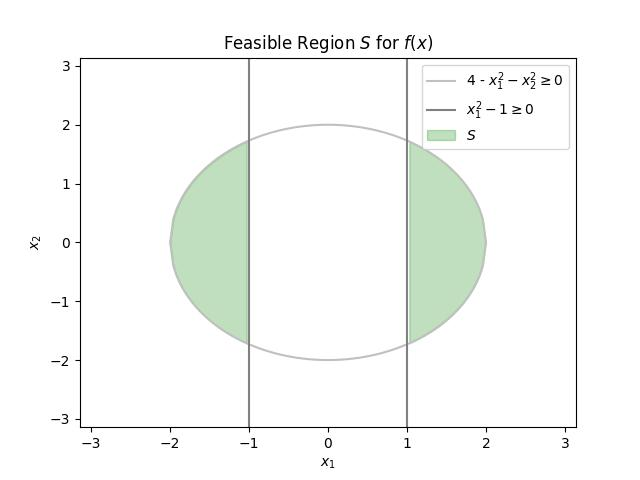
\includegraphics[width=0.9\textwidth]{problem_2.jpg}
    \caption{Feasible region $S$ (green)}
  \end{figure}

  Observe that $f(x) = x_1$ is minimized when $x_1$ attains its minimum value within the feasible region; from the above
  plot, we see that this occurs at $x = (-2, 0)$, which yields a local minimum of $f(x) = -2$. Moreover, $f(x)$ is not 
  bounded below (since it is linear), and so no global minimum of $f$ exists.
  \ \\
\end{solution}